\section{Data Distributions Across States}\label{sec:comparative-distribution}

This section focuses on the differences in the distribution of measured internet connectivity as a means of demonstrating how the different methods vary in their results. Building off the \kde charts from other chapters, we can filter to each state and plot the distributions of each of the methods in order to compare and contrast them.

Because the different methods use different metrics --- speed-of-light efficiency for traceroutes, time to load data from the top 50 website for site ping, and \rtt between \dns server for \dns cache manipulation --- there has to be some re-scaling of an $x$ axis to show a proper distribution. Traceroute data is reported as a fractionless scalar from 0-1, while site ping and \dns cache manipulation reports data in units of milliseconds; if graphed together without adjustment, one or the other would not even be visible. Consequently, all charts in this section are based on simple normalization by maximum value recorded across the \us. The \dns and site ping $x$ axes have been inverted for ease of understanding, so higher along the $x$ axis should always be interpreted as better.

As there are 51 charts total only a few are listed here, intended to provide the best evidence for the different observations about the distributions:

\paragraph{Site ping is the most extreme} Across all \kde charts for all graphs, data from traceroutes and \dns cache manipulation tend to agree with each other (although spread differs). However, site ping consistently reports values near the best possible value on these normalized axes, as demonstrated in \cref{fig:comparative_tn_dist}. The peak for traceroute data (referred to as just \caida on the charts) is sharper than \dns but close to its median value. In comparison, the peak for site ping is incredibly sharp and narrow, and focused over the 0.95-1.0 range.

% \begin{figure}[h]
\begin{wrapfigure}[16]{R}{0.55\textwidth}
    \centering
    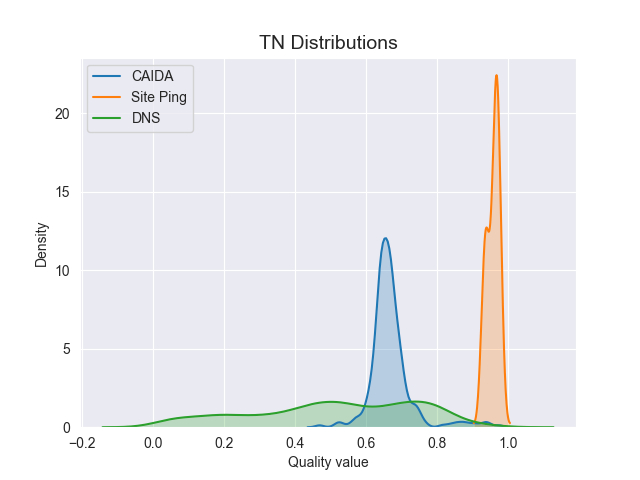
\includegraphics[width=0.55\textwidth]{comparative/state_dists/TN_dist.png}
    \caption{Tennessee data distributions}
    \label{fig:comparative_tn_dist}
\end{wrapfigure}
% \end{figure}

This should not be taken as an indicator that site ping reports consistently good quality, but that there are less common instances where it reports \textit{exceptionally} poor. The fact that its distribution is centered over high values is an artifact of normalizing by maximum value (and inverting) -- it means that somewhere to the far left, there's a small group of data points with poor connectivities, just not enough to be seen on the \kde charts. Keep in mind, this is \textit{after} z-score filtering to eliminate outliers.

Put more concisely: the worst connectivity reported by site ping are dramatically worse than the worst of either \dns or \caida data, even though on average it reports good connectivity.

\paragraph{DNS data has higher spread than traceroute data} In all charts, \dns cache manipulation data shows a much larger spread than traceroute data does. For instance, in \cref{fig:comparative_il_dist} we see consistent centering around the same point (approximately 0.65-0.7) for \textit{all} measures\footnote{Interestingly we see a smaller peak for site ping data at that point too. This helps confirm the prior theory that there is a small subset of poor-connectivity site ping data points.}, with traceroute and site ping showing roughly the same spread, but with \dns much more spread out.

% \begin{figure}[hb]
\begin{wrapfigure}[17]{L}{0.55\textwidth}
    \centering
    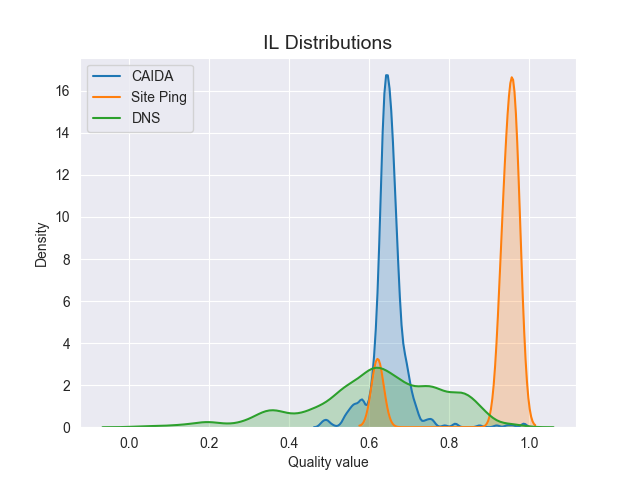
\includegraphics[width=0.55\textwidth]{comparative/state_dists/IL_dist.png}
    \caption{Illinois data distributions}
    \label{fig:comparative_il_dist}
\end{wrapfigure}
% \end{figure}

There's a fairly simple explanation for this, having to do with the way data was collected. As described in \cref{sec:dns_design_collection_stages} the \dns method involves taking several measurements and performing subtraction operations between them to determine a final value. Since each measurement has a margin of error (e.g. $\pm5$ ms), and error adds up with each addition or subtraction operation, it's only natural to see a wide distribution of data.

The downside to this, of course, is that aggregate measurements -- like those displayed in the state distributions charts -- are vulnerable to a wide spread. This makes it more statistically challenging to draw comparisons between states, for instance, as represented in various indistinguishability graphs across \crefrange{sec:caida}{sec:dns}.

\paragraph{Site ping is more likely to be bimodal; traceroute is typically unimodal}

Although not all \kde charts show it as strongly, site ping distributions are far more likely to be strongly bimodal. In contrast, traceroute data is almost always unimodal, although with occasional ripples on the outer edges of the distribution. \Cref{fig:comparative_ri_dist} is a good example of this behavior.

% \begin{figure}
\begin{wrapfigure}[14]{L}{0.55\textwidth}
    \centering
    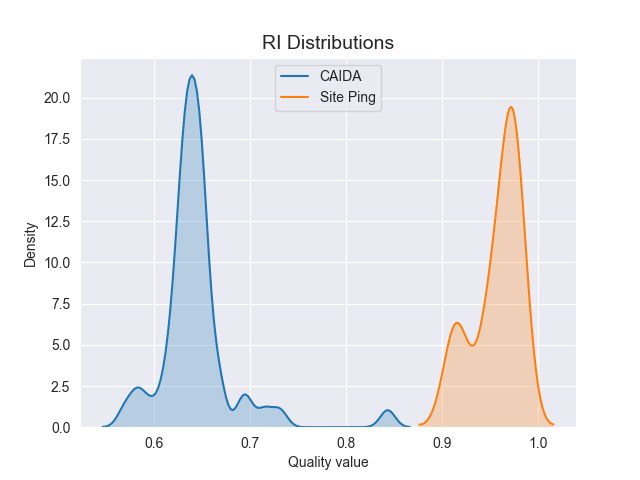
\includegraphics[width=0.55\textwidth]{comparative/state_dists/RI_dist.png}
    \caption{Rhode Island data distributions}
    \label{fig:comparative_ri_dist}
\end{wrapfigure}
% \end{figure}

The reasons for this are not entirely clear. \Cref{fig:caida_rtt_distribution}, the global \kde chart for all traceroute data in \cref{sec:caida_results}, shows an unusual, \textit{very} weakly bimodal distribution, but not an especially spread-out one. It may be that the occasional leftward peaks seen in site ping data area again due to the hypothesized greater-extremes from earlier before, but it's difficult to quantify.
